%%%%%%%%%%%%%%%%%%%%%%%%%%%%%%%%%%%%%%%%%%%%%%%%%%%%%%%%%%%%%%%%%%%%%%
% Lớp 11 | Quan hệ vuông góc trong không gian | Góc giữa đường thẳng và mặt phẳng. Góc nhị diện
% Dạng 1H8?6-5: Khoảng cách giữa điểm - mặt phẳng, biết trước góc (𝑑, (𝑃))
% Số câu: 8  (sinh tự động bởi tach_cau.py; từ nay thầy sửa trực tiếp file này)
%%%%%%%%%%%%%%%%%%%%%%%%%%%%%%%%%%%%%%%%%%%%%%%%%%%%%%%%%%%%%%%%%%%%%%

%%%%%%%%%%%%%%%% ĐÚNG/SAI %%%%%%%%%%%%%%%%

% nguồn: Ok_dungsai_lop11_Lan1
\begin{ex}%[1H8V6-5]%[ma:64755d08]
 Cho hình chóp $S.ABCD$ có đáy là hình vuông cạnh $a$. Biết $SA$ vuông góc với mặt phẳng đáy và $SA=a\sqrt{3}$. Vẽ đường cao $AH$  của tam giác $SAB$. Vẽ đường cao $AK$ của tam giác $SAD$. Khi đó, các mệnh đề sau \textbf{ĐÚNG} hay \textbf{SAI} ?
  \choiceTF
   {\True $BC\perp AH$}
  {\True Khoảng cách từ $A$ đến mặt phẳng $(SBC)$  bằng $\dfrac{a\sqrt{3}}{2}$}
  {Khoảng cách từ $A$ đến mặt phẳng  $(SBD)$ bằng $\dfrac{a\sqrt{2}}{7}$}
   {Khoảng cách từ $C$ đến mặt phẳng $(AHK)$ bằng $\dfrac{a\sqrt{5}}{5}$}
 \loigiai{ 
  \begin{center}
   \begin{tikzpicture}[scale=1,font=\footnotesize,line join=round,line cap=round,>=stealth]
      \path
      (0,3) coordinate[label=left: S]  (S)
      (0,0) coordinate[label=left: A]  (A)
      (2,-1)  coordinate[label=right: C] (C)
      (4,0)  coordinate[label=right: D] (D)
      (-2,-1) coordinate[label=left:  B] (B)
      ($(B)!.5!(D)$) coordinate[label=below: O]  (O)
      ($(B)!.4!(S)$) coordinate[label=below:  H] (H)
       ($(D)!.4!(S)$) coordinate[label=below: K] (K);
     \draw  (D)--(C)--(B);
     \draw[dashed] (B)--(A)--(D); 
     \draw[dashed]  (A)--(C)
      (D)--(B); 
      \draw[dashed] (S)--(A);
     \draw (B)--(S)--(C) 
       (D)--(S);
     \draw[dashed]  (A)--(K)
       (A)--(H);
      \draw[dashed] (A)--(S);
    \end{tikzpicture}
  \end{center}
  \begin{itemchoice}
    \itemch Đúng.
   Ta có $\heva{&BC\perp SA(\text{do}  SA\perp (ABCD) \\ &BC\perp AB} \Rightarrow BC\perp (SAB)\Rightarrow BC\perp AH$
    \itemch Đúng.
   Ta có $BC\perp AH$ mà $SB\perp AH$ nên  $AH\perp (SBC)$ hay $\mathrm{d}(A,(SBC))=AH$.
   Tam giác $SAB$ vuông tại $A$  có đường cao $AH$ nên
    \[\dfrac{1}{AH^2}=\dfrac{1}{AB^2}+\dfrac{1}{SA^2} \Rightarrow AH=\dfrac{AB\cdot SA}{\sqrt{AB^2+SA^2}}=\dfrac{a\cdot a\sqrt{3}}{\sqrt{a^2+3a^2}}=\dfrac{a\sqrt{3}}{2}.\]
    Vậy $\mathrm{d}(A,(SBC))=AH=\dfrac{a\sqrt{3}}{2}$.
   \itemch Sai. 
   Gọi $O$ là tâm hình vuông  $ABCD$ thì $AO\perp BD$.
    Ta lại có $SA\perp BD$ nên $BD\perp (SAC).$ $ \qquad (*)$
   Kẻ đường cao $AE$ của $\triangle SAO$ thì  $AE\perp BD$ (do $(*)$).
    Vậy $AE\perp (SBD)$ hay $\mathrm{d}(A,(SBD)=AE$.
   Ta có $AC=a\sqrt{2}$ (đường  chéo hình vuông), suy ra $OA=\dfrac{AC}{2}=\dfrac{a\sqrt{2}}{2}$.
   Tam giác $SAO$ vuông tại $A$ có $AE=\dfrac{SA\cdot AO}{\sqrt{SA^2+AO^2}}=\dfrac{a\sqrt{3} \cdot \dfrac{a\sqrt{2}}{2}}{\sqrt{3a^2+\dfrac{2a^2}{4}}}=\dfrac{a\sqrt{21}}{7}$. 
   Vậy $d(A,(SBD))=AE=\dfrac{a\sqrt{21}}{7}$. 
   \itemch  Sai.
   Ta chứng minh được $AK\perp (SCD)$. Khi đó:  $\heva {&SC\perp AH \\ &SC\perp AK} \Rightarrow SC\perp (AHK)$.
   Gọi $F=SC\cap  (AHK)$ thì $SC\perp AF$.
    Khi đó: $\mathrm{d}(C,(AHK))=CF$.
   Ta có $SC=\sqrt{SA^2+AC^2}=\sqrt{3a^2+2a^2}=a\sqrt{5}$. 
   Tam giác $SAC$ vuông tại $A$  có đường cao $AF$ nên:
   \[CF\cdot  CS=AC^2\Rightarrow CF=\dfrac{AC^2}{CS}=\dfrac{2a^2}{a\sqrt{5}}=\dfrac{2a\sqrt{5}}{5}.\]
   Vậy  $\mathrm{d}(C,(AHK))=CF=\dfrac{2a\sqrt{5}}{5}$
  \end{itemchoice}
 } 
\end{ex}

% nguồn: Ok_dungsai_lop11_Lan1
\begin{ex}%[1H8V6-5]%[ma:e2a36546]
 Cho  hình chóp đều $S.ABC$ có cạnh đáy bằng $a$, gọi $O$ là tâm của đáy và $SO=\dfrac{a\sqrt{3}}{3}$. Khi đó, các mệnh đề sau \textbf{ĐÚNG} hay \textbf{SAI} ?
 \choiceTF 
   {$AO=\dfrac{a\sqrt{3}}{2}$}
  {\True  $\mathrm{d}(O,SA)=\dfrac{a\sqrt{6}}{6}$}
  {\True Kẻ đường cao $AI$ của tam  giác $ABC$, khi đó: $OI=\dfrac{a\sqrt{3}}{6}$}
   {$\mathrm{d}(O,(SBC))=\dfrac{a\sqrt{15}}{12}$}
 \loigiai{ 
  \begin{center}
   \begin{tikzpicture}
     \path 
      (2.2,3) coordinate[label=left: S]  (S)
      (0,0) coordinate[label=above left: A]  (A)
      (5,0)  coordinate[label=right: C] (C)
      (2,-2) coordinate[label=left: B] (B) 
       ($(A)!.5!(B)$) coordinate (H)
      ($(C)!.5!(B)$)  coordinate (K)
      ($(C)!2/3!(H)$)  coordinate[label=below: O] (O);
     \draw  (S)--(A)--(B)--(C)
       (S)--(B)
       (S)--(C);
     \draw[dashed] (A)--(C) 
       (A)--(K)
      (C)--(H) 
      (S)--(O); 
    \end{tikzpicture}
  \end{center}
  \begin{itemchoice}
   \itemch  Sai.
   Kẻ đường cao $AI$ của tam giác  $ABC$, ta có $O$ thuộc $AI$.
   Trong mặt phẳng $(SAI)$, dựng $OH\perp SA$ tại $H\Rightarrow  \mathrm{d}(O,SA)=OH$.
   Tam  giác $ABC$ đều cạnh $a$ nên $AO=\dfrac{2}{3} AI=\dfrac{2}{3} \cdot \dfrac{a\sqrt{3}}{2}=\dfrac{a\sqrt{3}}{3}=SO$.
    \itemch Đúng.
   Tam giác  $SAO$ vuông cân tại $O$ nên $OH=\dfrac{SA}{2}=\dfrac{\dfrac{a\sqrt{3}}{3} \cdot
    \sqrt{2}}{2}=\dfrac{a\sqrt{6}}{6}$.
   Vậy  $\mathrm{d}(O,SA)=OH=\dfrac{a\sqrt{6}}{6}.$
   \itemch  Đúng.
   Ta có $OI=\dfrac{AI}{3}=\dfrac{\dfrac{a\sqrt{3}}{2}}{3}=\dfrac{a\sqrt{3}}{6}$. 
   \itemch Sai. 
   Ta xét khoảng cách từ $O$ đến mặt bên $(SBC)$. 
   Kẻ  đường cao $OK$ của tam giác $SOI$. \hfill{(1)}
   Ta có $\heva{&BC\perp SO(\text{ do } SO\perp (ABC)) \\& BC\perp  AI} \Rightarrow BC\perp (SAI)\Rightarrow BC\perp OK$.\hfill{(2)}
   Từ $(1)$ và $(2)$ suy ra $OK\perp  (SBC)$ hay $OK=d(O,(SBC))$.
   Tam giác  $SOI$ vuông tại $O$ có đường cao $OK$ nên
   \[\dfrac{1}{OK^2}=\dfrac{1}{SO^2}+\dfrac{1}{OI^2}  \Rightarrow OK=\dfrac{SO\cdot OI}{\sqrt{SO^2+OI^2}}=\dfrac{\dfrac{a\sqrt{3}}{3} \cdot \dfrac{a\sqrt{3}}{6}}{\sqrt{\dfrac{3a^2}{9}+\dfrac{3a^2}{36}}}=\dfrac{a\sqrt{15}}{15}\]
   Vậy $\mathrm{d}(O,(SBC))=OK=\dfrac{a\sqrt{15}}{15}$. 
  \end{itemchoice}
 } 
\end{ex}

% nguồn: Ok_dungsai_lop11_Lan1
\begin{ex}%[1H8V6-5]%[ma:25ccb844]
 Cho hình chóp $S.ABC$ có đáy là tam giác $ABC$ vuông tại  $B$ có $AB=1$,\quad \, \(\widehat{ACB}=30^{\circ}\). Biết $SA$ vuông góc với mặt đáy và $SA=2$. Gọi $H$ là hình chiếu của $A$ trên $SB$. Khi đó, các mệnh đề sau \textbf{ĐÚNG} hay \textbf{SAI} ?
  \choiceTF
   {\True $\mathrm{d}(A,SB)=AH$}
   {$\mathrm{d}(B,(SAC))=\dfrac{\sqrt{3}}{3}$}
  {\True  $BC=\sqrt{3}$}
  {Thể tích  khối chóp $S.ABC$ bằng $\dfrac{\sqrt{3}}{6}$}
 \loigiai{ 
  \begin{center}
   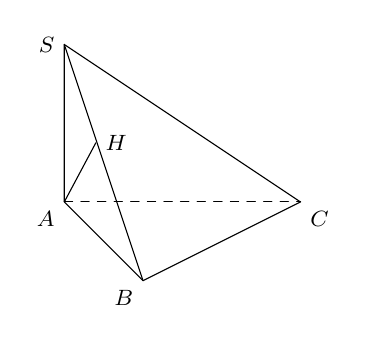
\begin{tikzpicture}[scale=1,font=\footnotesize,line join=round,line cap=round,>=stealth]
     \draw (0,0)--(1,-1)--(3,0)--(0,2)--cycle (0,0)--(.4,0.75); 
     \draw[dashed] (0,0)--(3,0); 
     \draw (0,2)--(1,-1); 
     \node[below left]  at (0,0) {$A$};
     \node[below left]at (1,-1)  {$B$};
     \node[below right]at (3,0) {$C$}; 
      \node[left]at (0,2) {$S$};
     \node[right]at (0.4,0.75)  {$H$};
    \end{tikzpicture}
  \end{center}
  \begin{itemchoice}
   \itemch Đúng. 
   Vì $AH\perp SB$ nên  $\mathrm{d}(A,SB)=AH$.
   Tam giác $SAB$ vuông tại $A$, đường cao $AH$  nên $\dfrac{1}{AH^2}=\dfrac{1}{SA^2}+\dfrac{1}{AB^2}$
   \[\Rightarrow AH=\dfrac{SA\cdot AB}{\sqrt{SA^2+AB^2}}=\dfrac{2\cdot  1}{\sqrt{2^2+1^2}}=\dfrac{2\sqrt{5}}{5}.\]
    \itemch Sai.
   Trong mặt phẳng $(ABC)$,  kẻ $BI\perp AC$ tại $I$.
   Mặt khác  $BI\perp SA$ (do $SA\perp (ABC)$, $BI\subset (ABC)$.
   Vì vậy  $BI\perp (SAC)$ hay $d(B,(SAC)=BI$.
   Tam  giác $ABI$ vuông tại $I$ có $\sin \widehat{BAC}=\dfrac{BI}{AB}$ $\Rightarrow BI=AB\cdot \sin 60^{\circ}=\dfrac{\sqrt{3}}{2}$.
   Vậy  $\mathrm{d}(B,(SAC))=BI=\dfrac{\sqrt{3}}{2}$.
    \itemch Đúng.
   Tam giác $ABC$ vuông tại $B$ có $\tan  \widehat{ACB}=\dfrac{AB}{BC}$ $\Rightarrow BC=\dfrac{AB}{\tan 30^{\circ}}=\sqrt{3}$.
   \itemch Sai. 
   Diện tích đáy hình  chóp là $S=S_{\triangle ABC}=\dfrac{1}{2} BA \cdot BC=\dfrac{\sqrt{3}}{2}$.
   Chiều  cao hình chóp $h=SA=2$.
   Thể tích  khối chóp $S.ABC$ là: $V_{S.ABC}=\dfrac{1}{3} Sh=\dfrac{1}{3} \cdot \dfrac{\sqrt{3}}{2} \cdot 2=\dfrac{\sqrt{3}}{3}$ (đơn vị thể tích).
  \end{itemchoice}
 } 
\end{ex}

% nguồn: Ok_dungsai_lop11_Lan1
\begin{ex}%[1H8V6-5]%[ma:db5ed7b6]
 Cho hình chóp $S.ABCD$ có đáy $ABCD$ là hình chữ nhật với $AB=2a$, $AD=a$. Hình chiếu của $S$ lên mặt phẳng $(ABCD)$ là trung điểm $H$ của $AB$ và $\widehat{SCH}=45^{\circ}$. Khi đó, các mệnh đề  sau \textbf{ĐÚNG} hay \textbf{SAI} ?
 \choiceTF 
  {\True  $BC\perp (SAB)$}
   {\True $\mathrm{d}(H,(SBC))=\dfrac{a\sqrt{6}}{3}$}
  {Gọi $K$ là trung điểm $CD$ khi đó $CD\perp (SHK)$} 
  {$\mathrm{d}(H,(SCD))=\dfrac{a\sqrt{6}}{2}$} 
  \loigiai{
  \begin{center}
   \begin{tikzpicture}
     \path 
       (-1,3) coordinate[label=left: S] (S)
       (0,0) coordinate[label=above right: A] (A)
      (2,-1) coordinate[label=right:  C] (C)
      (4,0) coordinate[label=right:  D] (D)
      (-2,-1) coordinate[label=left: B] (B) 
       ($(A)!.5!(B)$) coordinate[label=below right: H] (H);
      \draw (D)--(C)--(B);
     \draw[dashed] (B)--(A)--(D); 
     \draw[dashed] (S)--(A) 
       (S)--(H);
      \draw (B)--(S)--(C)
       (D)--(S);
    \end{tikzpicture}
  \end{center}
  \begin{itemchoice}
   \itemch Đúng. 
   Kẻ đường cao $HE$ trong tam giác  $SBH$. \hfill{(1)}
   Ta có $\heva{&BC\perp AB  \\ &BC\perp SH(\text{ do } SH\perp (ABCD)} \Rightarrow BC\perp (SAB)\Rightarrow BC\perp HE$. \hfill{(2)}
    \itemch Đúng.
   Từ (1) và (2)  suy ra $HE\perp (SBC)$ hay $\mathrm{d}(H,(SBC))=HE$.
   Tam giác $BCH$ vuông tại  $B$ có
   \[\begin{array}{ll} CH& {=\sqrt{BC^2+BH^2}} \\ {} & {=\sqrt{a^2+a^2}=a\sqrt{2}.}
  \end{array}\]
  Tam giác $SCH$ vuông  tại $H$ có
  \[\tan \widehat{SCH}=\dfrac{SH}{CH} \Rightarrow  SH=a\sqrt{2}.\;\]
  Tam giác $SBH$ vuông tại $H$ có đường cao $HE$  nên
  \[\begin{array}{ll}{\dfrac{1}{HE^2}} & {=\dfrac{1}{SH^2}+\dfrac{1}{BH^2}} \\[5pt] {\Rightarrow HE} & {=\dfrac{SH\cdot BH}{\sqrt{SH^2+BH^2}}} \\ {} & {=\dfrac{a\sqrt{2} \cdot a}{\sqrt{2a^2+a^2}}=\dfrac{a\sqrt{6}}{3}.}
 \end{array}\]
  Vậy $\mathrm{d}(H,(SBC))=HE=\dfrac{a\sqrt{6}}{3}$.
  \itemch Sai.
  Gọi $K$ là trung điểm $CD$ thì $HK$ là đường trung bình của hình chữ nhật $ABCD$ nên $HK\parallel BC\parallel AD\Rightarrow HK\perp CD$.
 Ta có $\heva{&CD\perp HK \\ &CD\perp SH} \Rightarrow CD\perp (SHK)$. 
  \itemch Sai.
 Kẻ đường cao $HI$ của tam giác $SHK$. 
 Ta có $\heva{&HI\perp SK \\ &HI\perp CD(\text{ do } CD\perp  (SHK),HI\subset (SHK))} \Rightarrow HI\perp (SCD)$.
 Tam giác $SHK$ vuông tại $H$ có  đường cao $HI$ nên
 \[\dfrac{1}{HI^2}=\dfrac{1}{SH^2}+\dfrac{1}{HK^2} \Rightarrow HI=\dfrac{SH\cdot HK}{\sqrt{SH^2+HK^2}}=\dfrac{a\sqrt{2}  \cdot a}{\sqrt{2a^2+a^2}}=\dfrac{a\sqrt{6}}{3}.\]
  Vậy $d(H,(SCD))=HI=\dfrac{a\sqrt{6}}{3}$.
 \end{itemchoice}
 }
\end{ex}

% nguồn: Ok_dungsai_lop11_Lan1
\begin{ex}%[1H8V6-5]%[ma:f6f8e582]
 Cho hình lăng trụ tam giác đều $ABC\cdot A' B' C'$ có cạnh đáy bằng $2a$, khoảng cách từ điểm $A'$ đến mặt phẳng $\left(AB' C'  \right)$ bằng $\dfrac{a\sqrt{3}}{2}$. Khi đó, các mệnh đề sau \textbf{ĐÚNG} hay \textbf{SAI}?
  \choiceTF
  {\True Trong mặt phẳng $\left(A' B' C' \right)$, kẻ  $A' H\perp B' C'$ tại $H$. Khi đó: $B'C'\perp (AA'H)$}
  {\True  $\mathrm{d}\left((ABC),\left(A' B' C' \right)\right)=a$}
  { Diện tích đáy  của lăng trụ là $a^2\sqrt{5}$}
   {\True Thể tích khối lăng trụ là $a^3\sqrt{3}$}
 \loigiai{ 
  \begin{center}
   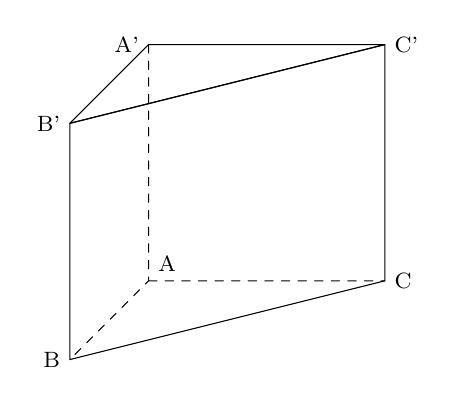
\begin{tikzpicture}[scale=1,font=\footnotesize,line join=round,line cap=round,>=stealth]
      \path
      (0,3) coordinate[label=left: A'] (A') 
       (0,0) coordinate[label=above right: A] (A)
      (3,0) coordinate[label=right:  C] (C)
      (3,3) coordinate[label=right: C']  (C')
      (-1,2) coordinate[label=left:  B'] (B')
      (-1,-1) coordinate[label=left: B]  (B);
     \draw  (A')--(B')--(C')--cycle;
      \draw (B)--(B')--(C')--(C)--cycle;
     \draw[dashed]  (A')--(A)--(B)
      (A)--(C); 
    \end{tikzpicture}
  \end{center}
  \begin{itemchoice}
    \itemch Đúng.
    Trong mặt phẳng $\left(A' B' C' \right)$, kẻ $A' H\perp B' C'$ tại $H$.
   Trong mặt phẳng $\left(AA'  H\right)$, kẻ $A' K\perp AH$ tại $K$. \hfill{(1)}
   Ta có  $\heva{&B'C'\perp A'H \\ &B'C'\perp AA'(do AA'\perp (A'B'C'))} \Rightarrow B'C'\perp (AA'H)$.
    \itemch Đúng.
   Ta có $ A'K\perp B'C'$.  \hfill{(2)}
   Từ $(1)$ và $(2)$ suy ra  $A' K\perp \left(AB' C' \right)$ hay $\mathrm{d}\left(A', \left(AB' C' \right)\right)=A' K=\dfrac{a\sqrt{3}}{2}$.
   Tam giác $A' B' C'$ đều có  đường cao $A' H=\dfrac{2a\cdot \sqrt{3}}{2}=a\sqrt{3}$.
   Tam giác $AA' H$ vuông  tại $A'$ có đường cao $A' K$ nên
   \[\dfrac{1}{A' K^2}=\dfrac{1}{A' H^2}+\dfrac{1}{A'  A^2} \Rightarrow \dfrac{1}{\dfrac{3a^2}{4}}=\dfrac{1}{3a^2}+\dfrac{1}{A' A^2} \Rightarrow A' A=a.\]
   \itemch  Sai.
   Hai mặt đáy lăng trụ song song với nhau  và có khoảng cách là
   $\mathrm{d}\left((ABC),\left(A' B'  C' \right)\right)=AA'=a.\;$
   Diện tích  đáy của lăng trụ (đáy là tam giác đều) là $S_{\Delta A' B' C'}=\dfrac{(2a)^2\sqrt{3}}{4}=a^2\sqrt{3}$
   \itemch Đúng. 
   Thể tích khối lăng trụ là: $V=AA'  \cdot S_{\Delta A' B' C'}=a\cdot a^2\sqrt{3}=a^3\sqrt{3}$ (đơn vị thể tích).
  \end{itemchoice}
  }
\end{ex}

% nguồn: Ok_dungsai_lop11_Lan1
\begin{ex}%[1H8V6-5]%[ma:7cfb581c]
 Cho hình chóp $S.ABC$ có mặt bên $(SAB)$  vuông góc với mặt đáy và tam giác $SAB$ đều cạnh $2a$. Biết tam giác $ABC$ vuông tại $C$ và cạnh $AC=a\sqrt{3}$. Khi đó, các mệnh đề sau \textbf{ĐÚNG} hay \textbf{SAI} ?
 \choiceTF 
  {\True $SH\perp (ABC)$} 
  {\True $\mathrm{d}(S,(ABC))=a\sqrt{3}$} 
  {$\mathrm{d}(C,(SAB))=\dfrac{a\sqrt{3}}{3}$} 
  {Thể  tích của khối chóp $S.ABC$ bằng $\dfrac{a^3}{6}$}
  \loigiai{
  \begin{center}
   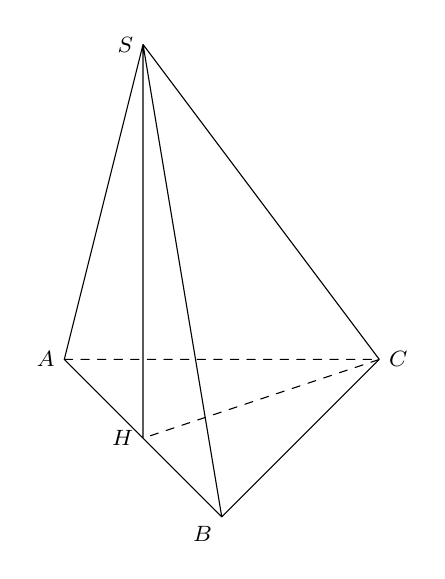
\begin{tikzpicture}[scale=1,font=\footnotesize,line join=round,line cap=round,>=stealth]
      \draw[dashed] (0,0)--(4,0)--(1,-1);
      \draw (0,0)--(2,-2)--(4,0)--(1,4)--(1,-1)
      (0,0)--(1,4)--(2,-2); 
     \node[right] at  (4,0) {$C$};
     \node[left] at  (0,0) {$A$};
     \node[below  left]at (2,-2) {$B$};
      \node[left]at (1,4) {$S$};
     \node[left]at  (1,-1) {$H$};
    \end{tikzpicture}
  \end{center}
  \begin{itemchoice}
   \itemch  Đúng.
    Gọi $H$ là trung điểm $AB$, mà tam giác $SAB$ đều nên $SH\perp AB$.
   Ngoài ra $(SAB)\perp (ABC)$ nên $SH\perp (ABC)$. 
   \itemch Đúng. 
   Ta có $\mathrm{d}(S,(ABC))=SH=\dfrac{2a\cdot  \sqrt{3}}{2}=a\sqrt{3}$ ( do tam giác $SAB$ đều cạnh $2a$).
   \itemch Sai. 
   Kẻ đường cao $CK$ của  tam giác $ABC$.
   Ta có  $\heva{&CK\perp AB\\ &CK\perp SH} \Rightarrow CK\perp (SAB)\Rightarrow \mathrm{d}(C,(SAB))=CK$.
    Xét tam giác $ABC$ vuông tại $C$ có
   \[BC=\sqrt{AB^2-AC^2}=\sqrt{4a^2-3a^2}=a;CK=\dfrac{CA\cdot  CB}{AB}=\dfrac{a\sqrt{3} \cdot a}{2a}=\dfrac{a\sqrt{3}}{2}.\]
    Vậy $\mathrm{d}(C,(SAB))=CK=\dfrac{a\sqrt{3}}{2}$.
   \itemch Sai. 
   Diện tích đáy hình  chóp là: $S_{\triangle ABC}=\dfrac{1}{2} AC\cdot BC=\dfrac{1}{2} a\sqrt{3} \cdot a=\dfrac{a^2\sqrt{3}}{2}$.
   Thể tích khối chóp là: $V_{S. ABC}=\dfrac{1}{3} SH\cdot S_{\triangle ABC}=\dfrac{1}{3} \cdot a\sqrt{3} \cdot  \dfrac{a^2\sqrt{3}}{2}=\dfrac{a^3}{2}$
  \end{itemchoice}
 } 
\end{ex}

% nguồn: Ok_dungsai_lop11_Lan1
\begin{ex}%[1H8V6-5]%[ma:95ff049d]
 Cho hình chóp $S.ABCD$ có đáy $ABCD$  là hình thang vuông tại $A$ và $D$. $SA$ vuông góc với mặt phẳng $(ABCD)$, $SA=AC$, $SC=2a$, $AB=2AD=2DC$.
  \choiceTF
  {\True $SA$ vuông góc với $BC$} 
  {\True Góc giữa đường thẳng $SC$ và mặt  phẳng $(ABCD)$ bằng $45^\circ$}
   {Góc giữa hai mặt phẳng $(SAC)$ và $(SBC)$ bằng $60^\circ$}
  {\True Khoảng cách  từ điểm $D$ đến mặt phẳng $(SBC)$ bằng $\dfrac{a}{2}$}
  \loigiai{
  \begin{center}
   \begin{tikzpicture}[line join=round,line cap=round,thick,scale=0.5]
     \coordinate (A)  at (0,0);
      \coordinate (D) at (-3,-3);
     \coordinate (I) at (7,0); 
     \coordinate  (C) at ($(D)+(I)-(A)$);
     \coordinate (S)  at ($(A)+(0,7)$);
     \coordinate (B) at ($(I)!-1!(A)$); 
      \coordinate (E) at ($(S)!0.5!(B)$);
     \coordinate (G) at  ($(C)!0.5!(B)$);
      \coordinate (H) at ($(E)!0.4!(G)$);
     \draw  (S)--(C)
      (S)--(D) 
       (C)--(D)
       (S)--(B)--(C)
       (E)--(G);
      \draw[dashed](I)--(S)--(A)--(C)
      (A)--(I)--(D) 
       (A)--(D)
       (I)--(B)
       (G)--(I)--(H)
      (C)--(I)--(E); 
     \pic [draw,angle radius=2mm] {right angle  = C--A--S} pic[draw,angle radius=2mm] {right angle = G--I--E} pic[draw,angle radius=2mm] {right angle = I--H--G};
      \foreach \i/\g in {S/90,A/180,I/-90,C/-90,D/-90,E/90,B/0,G/-90,H/0}{\draw[fill=black](\i) circle (0pt)
       ($(\i)+(\g:4mm)$) node[scale=1]{$\i$};}
    \end{tikzpicture}
  \end{center}
  \begin{itemchoice}
   \itemch Vì  $SA\perp(ABCD)\supset BC\Rightarrow SA\perp BC$.
   \itemch  $SA\perp (ABCD)\Rightarrow A$ là hình chiếu vuông góc của $S$ lên $(ABCD)\Rightarrow AC$ là hình chiếu vuông góc của $SC$ lên $(ABCD)\Rightarrow \left(SC,(ABCD)\right)=(SC,AC)=\widehat{SCA}$.\\
   Theo giả  thiết $\Delta SAC$ vuông cân tại $A\Rightarrow\widehat{SCA}=45^\circ$.
   \itemch $SC=(SAC)\cap (SBC)$. Gọi $I$ là trung điểm $AB$ theo giả thiết  ta có tam giác $\Delta ACB$ vuông cân tại $C$.\\
   Ta  có
   $\heva{& BC  \perp AC\\&BC\perp SA} \Rightarrow BC\perp (SAC)$.\\
   Do $BC\subset (SBC)\Rightarrow (SBC)\perp  (SAC)\Rightarrow \left((SAC),(SBC)=90^\circ\right)$.
   \itemch Gọi $G, E$ lần lượt là trung điểm của $BC, SB$  ta có $\heva{&IE\perp (ABCD)\\
   &IG\perp BC&}$ 
   và $EG$ là đường trung bình của  tam giác $\Delta SBC$.\\
   Ta có $DI\parallel BC\subset (SBC)\Rightarrow  DI\parallel (SBC)\Rightarrow{d_{(D,(SBC))}}=d_{(I,(SBC))}$.\\
    Ta lại có
   $\heva{&BC\perp  IG\\
    &BC\perp IE
   &}$ $\Rightarrow  BC\perp (IGE)$. Kẻ $IH\perp EG\Rightarrow IH\perp (SBC)\Rightarrow{d_{(I,(SBC))}}=IH$.\\
   Theo cách  gọi các điểm $G, E$ và giả thiết ta có $IE=IG=\dfrac{1}{2}SA\Rightarrow\Delta IEG$ vuông cân tại
   $I\Rightarrow IH=\dfrac{1}{2}EG=\dfrac{1}{2}\cdot  \dfrac{1}{2}SC=\dfrac{a}{2}\Rightarrow{d_{(D,(SBC))}}=\dfrac{a}{2}\cdot$
  \end{itemchoice}
 } 
\end{ex}


%%%%%%%%%%%%%%%% TRẢ LỜI NGẮN %%%%%%%%%%%%%%%%

% nguồn: Ok_TraLoiNgan_Lop11_Lan1
\begin{ex}%[1H8H6-5]%[ma:43d464ae]
	Cho hình  hộp chữ nhật $ABCD.A' B' C' D'$ có $AB=a$, $AD=2a$, $AA'=3a$. Tính góc phẳng nhị diện $\left[A',BD,A\right]$? (đơn vị đo góc là độ, làm tròn đến hàng phần chục)
	 \shortans{73,4}
	 \loigiai{
		\begin{center}
			\begin{tikzpicture}[scale=1,font=\footnotesize,line join=round,line cap=round,>=stealth]
					 \path
						(0,0) coordinate[label=left:  A] (A)
						(5,0)  coordinate[label=right: D] (D)
						(3,-2) coordinate[label=right: C] (C) 
						 (-2,-2) coordinate[label=left: B] (B)
						(0,4) coordinate[label=left: A'] (A') 
						(5,4)  coordinate[label=right: D'] (D')
						(3,2) coordinate[label=right:  C'] (C')
						 (-2,2) coordinate[label=left: B'] (B')
						($(B)!.4!(D)$) coordinate[label=below right: I] (I); 
					 \draw (A')--(B')--(C')--(D')--cycle (B')--(B)--(C)--(D)--(D')
						 (C)--(C');
					\draw[dashed]  (A')--(A)--(B)
						(A)--(D) 
						(B)--(D) 
						 (A)--(I);
				\end{tikzpicture}
		\end{center}
		Kẻ $AI\perp BD$.\\ 
		Mà $BD\perp A' A\Rightarrow BD\perp \left(AA' I\right)$.\\ 
		Ta  có
		\[\heva{&\left(A' BD\right)\cap (ABD)=BD \\ &\text{Trong  }(ABD),AI\perp BD \\ &\text{Trong }\left(A' BD\right),A' I\perp BD} \Rightarrow \left[A', BD,A\right]=\widehat{A {'}IA}.
		 \]
		 Ta có $AI=\dfrac{1}{\sqrt{\dfrac{1}{AB^2}+\dfrac{1}{AD^2}}}=\dfrac{1}{\sqrt{\dfrac{1}{a^2}+\dfrac{1}{(2a)^2}}}=\dfrac{2\sqrt{5}}{5} a$.\\
		Xét $\Delta  AA' I$ vuông tại $A$: $\tan \widehat{A' IA}=\dfrac{A' A}{AI}=\dfrac{3a}{\dfrac{2\sqrt{5}}{5} a}=\dfrac{3\sqrt{5}}{2} \Rightarrow \widehat{A' IA}\approx 73{,}4^{\circ}$.
	 }
\end{ex}
